\section{Oceanic surface layer}
\label{sec:OceanND_OSL}
We now interest ourselves to the discretization of an ocean
column and its surface layer.
If a \textit{two-sided} bulk is used then the
discretization of the oceanic surface layer can be derived
similarly to the discretization of the atmospheric surface
layer in Chapter \ref{ch:ND}.
\par
In the ocean modeling community, it is unusual to use
wall modeling at the surface. The Sea Surface Temperature
(SST) is often taken at the first grid level inside the
ocean: this corresponds to the assumption that 
the profiles are constant in the surface layer.
\cite{zeng_prognostic_2005} proposed a scheme to avoid this
issue for weather forecasting, climate modeling and
data assimilation.
%
\par
The goal of this section is to investigate the effects
of the surface layer discretization in a coupled situation.
We first (Section \ref{sec:ND_Ocean_differencesWithAtmosphere})
specify the differences between the ocean and
atmosphere models in use,
then focus on the incorporation of radiative fluxes in
Section \ref{sec:ND_Ocean_radiativeFluxes}.
Finally, Section \ref{sec:ND_Ocean_bulkRadiativeFluxes}
presents the sensitivity to the discretization of the
surface layer in the coupled setting.
\subsection{Differences with the atmosphere and derivation of
	a symmetric surface flux scheme}
\label{sec:ND_Ocean_differencesWithAtmosphere}
In this section, the numerical model of a stratified column
of ocean is described. The objective is to obtain a model
similar to the atmosphere while including the specificity
of the ocean.
In particular, the main changes compared to the atmosphere
model are:
\begin{itemize}
	\item the density which mainly affects the exchanges
		between ocean and atmosphere;
	\item the universal stability functions which are
		taken in \cite{large_similarity_2019};
	\item the vertical axis $z \leq 0$
		which is such that the surface corresponds to $z=0$;
	\item the time and space scales (the motion in the ocean
		is slower and smaller space steps are used with
		larger time steps).
\end{itemize}
\subsubsection{The Ocean model}
We describe here the continuous model in use for the ocean.
The equations for momentum, potential temperature and
turbulent kinetic energy in the inner domains are not changed
except that the geostrophic momentum is not included in the ocean:
\begin{equation}
	\begin{aligned}
	&(\partial_t + if) u - \partial_z (K_u \partial_z u) = 0
		,~~~~~ z \leq \delta_{o} \\
	&\partial_t \theta -\partial_z (\partial_z K_{\theta} \theta)
	= F_{\theta},~~~~~~~~~~~~~~ z \leq \delta_{o} \\
		&\partial_t e =
    \underbrace{\partial_z \left(K_e
    \partial_z e\right)}_{\text{diffusion}}
    + \underbrace{K_u ||\partial_z u||^2}_{\text{shear}} 
    - \underbrace{K_{\theta} N^2 }_{\text{buoyancy}}
    - \underbrace{c_{\epsilon}
    \frac{e^{3/2}}{l_{\epsilon}(z)}}_{\text{dissipation}}
	\end{aligned}
\end{equation}
$F_\theta = -\frac{\partial_z Q_{sw}}{\rho_{\rm o} C_p}$ is a
radiative forcing corresponding to the shortwave flux of a
diurnal cycle. As in the atmospheric case the buoyancy $N^2$ is
given by a linear equation of state
$N^2 = g \alpha \partial_z \theta$.
The mixing lengths follow the description in 
\ref{sec:ND_StratifiedCase_turbulentVisc}
except that $l_{up}$ and $l_{down}$ are swapped and the shear
is neglected in \eqref{eq:ND_StratifiedCase_lD80}.
%
\paragraph{Initialization and boundary conditions.}
At initialization, the TKE is set to $e=e_{\rm min}$, 
the temperature is set to a constant $\theta = 280 \; {\rm K}$
and the initial momentum is set to $u = 0 \; {\rm m}.{\rm s}^{-1}$.
At the bottom boundary,
$\partial_z u = 0$,
$\partial_z \theta = 0$ and $e=e_{\rm min}$.

\subsubsection{The surface boundary condition}
We derive here the surface flux "FV free" applied to the oceanic
column model. Let $k$ be the space index such that
$z_{k-1} < \delta_o \leq z_k$;
we note $\widetilde{u}, \widetilde{\theta}$
the averaged variables over the interval $(z_{k-1}, \delta_o)$.
In the case of the atmosphere column, equation
\eqref{eq:ND_StratifiedCase_relation_tilde_bar}
gives the relation between the averaged variables
$\overline{u}, \overline{\theta}$ over the volume $(z_{k-1}, z_{k})$.
The same relation can be written here:
\begin{equation}
\begin{aligned}
\label{eq:ND_Ocean_relation_tilde_bar}
\alpha_{o, u}\widetilde{u} = \overline{u}_{k-1/2} -
\widetilde{h}
	\left(\frac{\phi_{\delta}}{3} + \frac{\phi_{k-1}}{6}\right)
	\left(\alpha_{o, u} - \frac{\widetilde{h}}{h_{k-1/2}}\right)
	- (1 - \alpha_{o, u})u(0)\\
\alpha_{o, \theta}
\widetilde{\theta}
= \overline{\theta}_{k-1/2} -
	\widetilde{h}\left(\frac{{(\partial_z \theta)}_{\delta}}{3}
	+ \frac{{(\partial_z \theta)}_{k-1}}{6}\right)
	\left(\alpha_{o, \theta}-\frac{\widetilde{h}}{h_{k-1/2}}\right)
 - (1 - \alpha_{o, \theta})\theta_s
\end{aligned}
\end{equation}
with for $x = u, \theta$:
\begin{equation}
	\alpha_{o, x} = \frac{\widetilde{h}}{h_{k-1/2}} +
	\frac{\frac{1}{{h_{k-1/2}}}\int_{\delta_{o}}^{z_k} x(0) - x(z)
	dz}{x(0) - x(\delta_{o})}
\end{equation}
Appendix \ref{sec:ND_Ocean_stabilityFunctionIntegration}
details the derivation of the explicit formula of $\alpha_{o}$
with the oceanic universal stability functions.
Finally, the scheme at the first grid level above
the surface layer is:
\begin{equation}
	\label{eq:ND_Ocean_semiDiscreteEkmanEqFVfree}
	(\partial_t+if) \widetilde{u}
	= \frac{K_{u, \delta_o}\phi_{\delta_o}
	- K_{u,k-1} \phi_{k-1}}{\widetilde{h}}
\end{equation}
\begin{equation}
	\label{eq:ND_Ocean_semiDiscreteEkmanEqPTFVfree}
	\partial_t \widetilde{\theta}
	= \frac{K_{\theta, \delta_o}{(\partial_z \theta)}_{\delta_o} -
	K_{\theta,k-1} {(\partial_z \theta)}_{k-1}}{\widetilde{h}}
	+ \widetilde{F}_\theta 
\end{equation}
where for $x=u,\theta$:
\begin{equation}
	\label{eq:ND_Ocean_semiDiscreteEkmanEqPTFVfree}
	\widetilde{x} = \frac{1}{\alpha_{\rm o, x}(t)}
	\left(
	\overline{x}_{k-1/2} -
	\widetilde{h}(\frac{{(\partial_z x)}_{\delta_o}}{3} +
	\frac{{(\partial_z x)}_{k-1}}{6})
	\left(\alpha_{o, x}-\frac{\widetilde{h}}{h_{k-1/2}}\right)
	 - (1 - \alpha_{o, x})x(0)
	\right)
\end{equation}
In the surface layer, the hypothesis that the potential
temperature is quasi-stationary gives that
$\forall z > \delta_o, ~~
\partial_z \left(K_\theta \partial_z \theta \right)
= \frac{\partial_z Q_{sw}}{\rho_{\rm o} C_p}$.
The scheme uses as boundary conditions at the surface layer:
\begin{equation}
\label{eq:ND_Ocean_boundaryConditionFVfree}
\begin{aligned}
	K_{u,\delta_o} \phi_{\delta_o} &= \frac{\rho_{\rm a}}
	{\rho_{\rm o}}
	u_\star^2 e_\tau
	\\
	K_{\theta, \delta_o} (\partial_z \theta)_{\delta_o} &= 
	\frac{\rho_{\rm a} c_{\rm a}^p}{\rho_{\rm o} c_{\rm o}^p}
	\theta_\star u_\star - \frac{Q_{lw} + Q_{sw}(\delta_{o})}{\rho_{\rm o} c_{\rm o}^p}
  \end{aligned}
\end{equation}
where $c_{\rm a}^p$, $c_{\rm o}^p$ are the heat capacities
of air and water and
$Q_{lw}, Q_{sw}$ are defined in Section
\ref{sec:ND_Ocean_radiativeFluxes}.
The surface flux scheme is summarized in Figure
\ref{fig:ND_Ocean_nouvelle_dis_neutre}.
\begin{figure}
	\subimport{images/}{nouvelle_dis_neutre_ocean.pdf_tex}
	\caption{Surface layer scheme "FV free" in the ocean model}
	\label{fig:ND_Ocean_nouvelle_dis_neutre}
\end{figure}
As it will be explained
in Section \ref{sec:ND_Ocean_radiativeFluxes} this surface flux scheme
does not correctly take into account the radiative fluxes and the
interval $(\delta_o, z_k)$ needs an evolution equation for $\theta$.
\subsection{Radiative fluxes, another surface flux scheme}
\label{sec:ND_Ocean_radiativeFluxes}
We note $Q_{sw}$ and $Q_{lw}$ the shortwave and longwave (positive
downward) fluxes.
To include those fluxes in the
bulk formula, \cite{pelletier_two-sided_2021} introduced
a variable $\theta^\star_{o, \rm rad}$
that is similar to a friction scale but depends on $z$:
\begin{equation}
\theta_\star^{\rm rad}(z) =
	\theta_\star -
	\frac{Q_{sw}(z) + Q_{lw}}{u_{\star}\rho_{\rm a} c_{\rm a}^p}
\end{equation}
This variable is used instead of $\theta^\star_{a}$
in the ocean part of the two-sided bulk procedure
to include the radiative fluxes.
To be fully consistent between the computational domain and
the oceanic surface layer, the boundary condition for the temperature
should take into account the radiative fluxes: in
\eqref{eq:ND_Ocean_boundaryConditionFVfree} the flux
$K_\theta \partial_z \theta$ is exactly equal to
$\frac{\rho_{\rm a} c_{\rm a}^p}{\rho_{\rm o} c_{\rm o}^p}
\theta_\star^{\rm rad}(\delta_o) u_\star$.
Moreover, to avoid the integration of $Q_{sw}$
in the Finite Volume discretization,
we use an evolution equation
inside the surface layer despite the contradiction with
the quasi-stationarity.
% \myTD{
% 	Techniquement on a le flux, on pourrait intégrer $\partial_z \theta$.
% 	On fait pas ça parceque:
% 	- Ca serait compliqué déjà d'intégrer $Q_{sw}$ analytiquement
% 	- En vrai ça marche pas mal d'ensure l'equation d'evolution dans la SL ?
% 	Notons qu'avec une intégration propre du flux on aurait pas
% 	non plus de problème de conservation de temp potentielle
% 	Moreover, since the flux is now vertically varying in the oceanic
% surface layer there is an accumulation of the potential
% temperature during the day. To keep the conservation property
% of the Finite Volume discretization one cannot treat
% the surface layer implicitly for the potential temperature.
% }
%
% \par
% The bulk procedure is the one used in
% \citep{pelletier_two-sided_2021}.
% When computing
% $\frac{\kappa (\theta(\delta_a) - \theta(\delta_o))}
% 	{\theta_a^{\star}}$,
% 	we use:
% \begin{equation}
% 	\label{eq:ND_Ocean_skinbulk}
% 	\frac{\kappa (\theta(0) - \theta(\delta_o))}
% 	{\theta_o^{\star}} = (1 -
% 	\frac{Q_{lw}}{Q_H})
% 	\left(\ln (1 - \frac{\delta_o}{z_{\theta}}) -
% 	\psi_h(\frac{-\delta_o}{L_o})\right)
% 	- \frac{\lambda_\theta Q_{sw}(0)}
% 	{Q_H} E(\delta_o)
% \end{equation}
\par
%\subsubsection{Adding radiative fluxes: derivation without
%molecular sub-layer}
We neglect the molecular sub-layer and
integrate between $\delta_o$ and 0:
the flux at $z=0$ is
$K_\theta \partial_z \theta = \frac{Q_H - Q_{lw}}{\rho_{\rm o} c_{\rm o}^p}$
where $Q_H = \theta_o^\star u_o^\star \rho_{\rm o} c_{\rm o}^p$
\begin{equation}
\label{eq:evolEqOSL}
h_{osl}\partial_t \overline{\theta}_{osl} =
	\frac{Q_H - Q_{lw}}{\rho_{\rm o} c_{\rm o}^p}
- \left. K_\theta \partial_z \theta 
\right|_{\delta_{o}}
- h_{osl}\int_{\delta_o}^0
	\frac{\partial_z Q_{sw}}{\rho_{\rm o} c_{\rm o}^p} dz
\end{equation}
where $h_{osl} = |\delta_o|$
is the size of the surface layer and
$\overline{\theta}_{osl}$ is the average potential
temperature in the surface layer.
We will use the following reconstruction of $\theta$
inside the SL (taken from \citep{zeng_prognostic_2005}
where the molecular surface layer was neglected to simplify
the expressions):
\begin{equation}
	\label{eq:ND_Ocean_reconstructionSimpleTheta}
    \theta(z) = \theta_s -
    \left(\frac{z}{\delta_{o}}\right)^\nu \left( \theta_s - 
    \theta_{\delta_o}\right)
\end{equation}
where $\nu$ is a constant parameter that can be set to 1 to
recover a linear reconstruction of $\theta(z)$.
\cite{zeng_prognostic_2005} choose $\nu=0.3$ and argue that
the choice of $\nu$ is linked to the size of the molecular
sub-layer.
We formulate the reconstruction in terms of $\overline{\theta}_{osl}$
and $\left.\partial_z \theta\right|_{\delta_o}$:
\begin{equation}
    \overline{\theta}_{osl} = \frac{1}{\nu+1}
    (\theta_{\delta_o} + \nu \theta_s)
, ~~~ \left.\partial_z \theta \right|_\delta
= \frac{\nu}{h_{osl}} (\theta_s - \theta_{\delta_o})
\end{equation}
We get that the surface temperature
is $\theta_s = \overline{\theta}_{osl}
+ \frac{h_{osl}}{\nu(\nu+1)} \partial_z \theta$ and
the difference of temperature between
the surface and the bottom of the surface layer is
$\theta_s - \theta_{\delta_o} = 
\frac{h_{osl}}{\nu}\partial_z \theta$:
\begin{equation}
    \theta(z) = \overline{\theta}_{osl} +
    \frac{h_{osl}}{\nu} \partial_z \theta_{\delta_o} \left(
    \frac{1}{\nu+1} - \left(\frac{z}{\delta_{o}}\right)^\nu
\right)
\end{equation}
\begin{remark}
It would be possible to consider that $\overline{\theta}_{osl}$ is
the average in an interval $(\delta_o, z_k)$.
However the radiative forcing would affect each individual cell
inside the surface layer, leading to a contradiction with the simple
reconstruction \eqref{eq:ND_Ocean_reconstructionSimpleTheta}
of the surface layer.
We instead assume here that $|\delta_{o}| < |z_{-1}|$.
\end{remark}
Let us assume now that  $\theta(z)$ is a quadratic spline between
$z_{-1}$ and $\delta_o$.
Using the continuity at $z=\delta_o$ and Chasles' relation,
we link the surface layer profile with the spline:
\begin{equation}
\underbrace{
    \overline{\theta}_{osl} -
    \frac{h_{osl}}{\nu+1}\left. \partial_z \theta
    \right|_{\delta_o}}_{\theta(\delta_o^{+})}
    =
    \underbrace{
    \widetilde{\theta}
    + \frac{\widetilde{h}}{3}
    \left.\partial_z \theta\right|_{\delta_o}
    + \frac{\widetilde{h}}{6}
	\left.\partial_z \theta\right|_{z_{-1}}}_{
	\theta(\delta_o^{-})}
	,
    ~~~~
	\underbrace{
    h_{-1/2} \overline{\theta} = 
    h_{osl}\overline{\theta}_{osl} +\widetilde{h}
    \widetilde{\theta}}_{
    \int_{z_{-1}}^{0}\theta(z) dz
    }
\end{equation}
The reconstruction for $|z|<|\delta_o|$ (inside the surface layer) is hence
\begin{equation}
    \theta(z) =
    \overline{\theta}_{-\frac{1}{2}}
    +
	\left(\frac{h_{osl}\widetilde{h}}{-z_{-1}(\nu+1)} +
	\frac{\widetilde{h}^2}{-3 z_{-1}}
    +
    \frac{h_{osl}}{\nu}\left(
    \frac{1}{\nu+1} + \left(\frac{z}{h_{osl}}
    \right)^\nu
    \right)\right) \partial_z \theta_{\delta_o}
    +
	\left(\frac{\widetilde{h}^2}{-6 z_{-1}}\right)
    \partial_z \theta_{-1}
\end{equation}
for $|\delta_o| < |z| < |z_{-1}|$
(in the quadratic region) we have
\begin{equation}
    \theta(z) =
        \widetilde{\theta}
        +
        \left(
        z-\delta_o + 
        \frac{(z-\delta_o)^2}{2\widetilde{h}}
        + \frac{\widetilde{h}}{3}
        \right)\partial_z \theta_{\delta_o}
        +
        \left(
        \frac{\widetilde{h}^2 - 
        3(z-\delta_o)^2}{6 \widetilde{h}}
        \right)\partial_z \theta_{-1}
\end{equation}
where $\widetilde{\theta}$ is computed with
\begin{equation}
\label{eq:formulaTildeTheta}
\widetilde{\theta} = \overline{\theta}_{-1/2}
	-\frac{\delta_o}{z_{-1}}\left(
\frac{h_{osl}}{\nu+1} + \frac{\widetilde{h}}{3}
\right)\partial_z \theta_{\delta_o}
	- \frac{\widetilde{h}\delta_o}{6z_{-1}}
\partial_z \theta_{-1}
\end{equation}
The continuity equation at $z_{-1}$
uses $\widetilde{h}$
as the space step:
\begin{equation}
    \widetilde{\theta}
    - \frac{\widetilde{h}}{3}
    \partial_z \theta_{-1}
    - \frac{\widetilde{h}}{6}
    \partial_z \theta_{\delta_o}
    = \overline{\theta}_{-3/2}
    + \frac{\widetilde{h}}{3}
    \partial_z \theta_{-1}
    + \frac{\widetilde{h}}{6}
    \partial_z \theta_{-2}
\end{equation}
The evolution equation of the first volume is:
\begin{equation}
h_{-\frac{1}{2}}\partial_t
\overline{\theta}_{-\frac{1}{2}} =
	\frac{Q - Q_{lw}}{\rho_{\rm o} c_{\rm o}^p}
- K_{\theta, -1} \partial_z \theta_{-1}
- h_{-\frac{1}{2}}\int_{z_{-1}}^0
	\frac{\partial_z Q_{sw}}{\rho_{\rm o} c_{\rm o}^p} dz
\end{equation}
We need a last equation to close the system.
Starting from \eqref{eq:formulaTildeTheta}, we get
\begin{equation}
\partial_t
\left(
\widetilde{h}\overline{\theta}_{-1/2}
	-\frac{\delta_o}{z_{-1}}\left(
\frac{\widetilde{h}h_{osl}}{\nu+1} + \frac{\widetilde{h}^2}{3}
\right)\partial_z \theta_{\delta_o}
	- \frac{\widetilde{h}^2\delta_o}{6z_{-1}}
\partial_z \theta_{-1}
\right)
	= K\partial_z \theta_{\delta_o}-
K\partial_z \theta_{-1}
- \widetilde{h}
\int^{\delta_o}_{z_{-1}}
	\frac{\partial_z Q_{sw}}{\rho_{\rm o} c_{\rm o}^p} dz
\end{equation}
Note that the reconstruction we are using is not differentiable
in $z=0$.
If greater regularity is needed, it is possible to link
the reconstruction with a proper modeling of the molecular sub-layer
(e.g. $\rho_{\rm o} c_{\rm o}^p K_{mol} \partial_z \theta(z) =
Q - Q_{lw} - \int_z^0 \partial_z Q_{sw}(z')dz'$ for $|z|<<|\delta_o|$)
% It is hence more appealing to take into account
% the molecular sublayer to add some regularity to the solution.
% \subsubsection{Oceanic surface flux scheme with molecular sublayer}
% We now imitate the previous derivation, using a more regular
% reconstruction for $\theta(z)$ inside the surface layer:
% we take exactly the reconstruction used by
% \cite{zeng_prognostic_2005}: let $d << |\delta_o|$ be the
% depth of the molecular sublayer:
% \begin{equation}
% 	\theta(z) = \theta_{-d} -
% 	\left(\frac{z+d}{\delta_o + d}\right)^\nu
% 	\left(\theta_{-d} - \theta_{\delta_o}\right)
% \end{equation}
% where the temperature at the bottom of the molecular sublayer
% $\theta_{-d}$ is linked to the surface temperature through an
% integration of
% $K_{mol}\partial_z \theta = \frac{Q-Q_{lw}}{\rho_{\rm o} c_{\rm o}^p} -
% \frac{1}{\rho_{\rm o} c_{\rm o}^p}\int_{-d}^0\partial_z Q_{sw}(z)dz$:
% \begin{equation}
% 	\theta_{-d} = \theta_s - \frac{d}{\rho_{\rm o} c_{\rm o}^p K_{\theta, mol}}
% 	\left(
% 	\frac{Q-Q_{lw} - Q_{sw}(0)f_s}{\rho_{\rm o} c_{\rm o}^p}
% 	\right).
% \end{equation}
% $f_s$ is here the fraction of solar radiation absorbed in the
% sublayer, described in \cite{zeng_prognostic_2005}.
% $d$ can be parametrized by $u_\star$ and the fluxes.
\subsection{Sensitivity to the discretization
	of the surface layers}
\label{sec:ND_Ocean_bulkRadiativeFluxes}
\myTD{TODO commenter figures}
Figure \ref{fig:OceanND_OSL_Forced}
show the profiles obtained in wind and
potential temperature with several discretisations.
As in Chapter \ref{ch:ND} a high resolution simulation
where every cell is divided into three cells
is also performed.
One can see that the high resolution
is far from the normal simulation only in the "FV free"
discretization.

Figure \ref{fig:OceanND_OSL_Coupled}
is the same as Figure 
\ref{fig:OceanND_OSL_Forced} except that the ocean column is coupled
with the atmosphere column described in Chapter \ref{ch:ND}.
\begin{figure}
	\centering
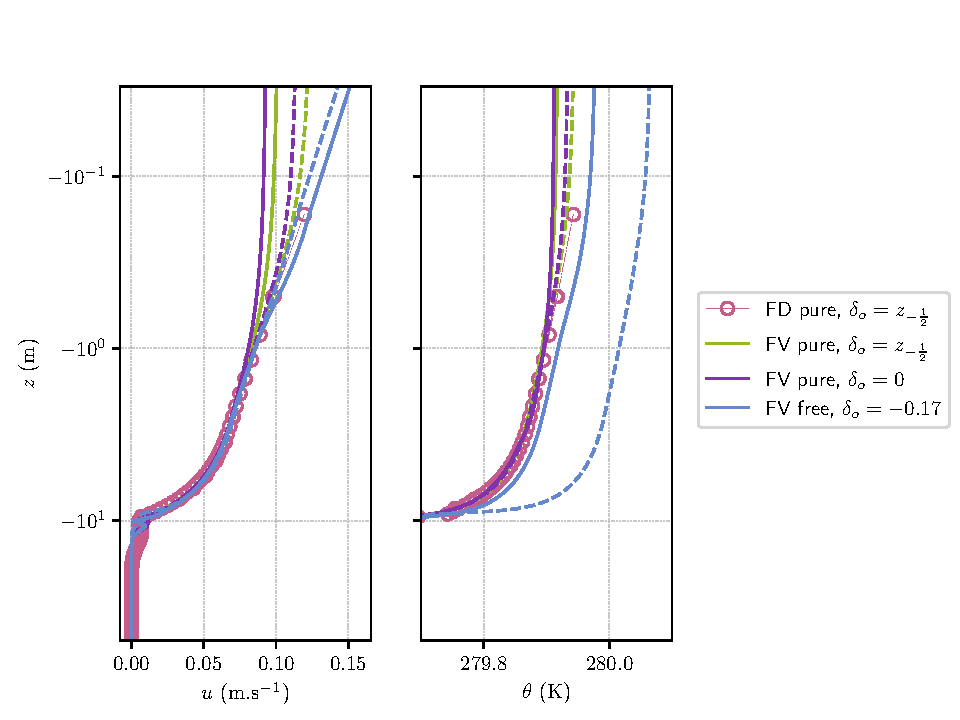
\includegraphics[scale=0.6]{images/oce_Forced.pdf}
	\caption{Forced case: dashed lines indicate
	a high resolution simulation and solid lines
	show the normal simulation. Numerical parameters
	are the same as in \S \ref{sec:ND_Consistency_Coupled}.}
	\label{fig:OceanND_OSL_Forced}
\end{figure}
\begin{figure}
	\centering
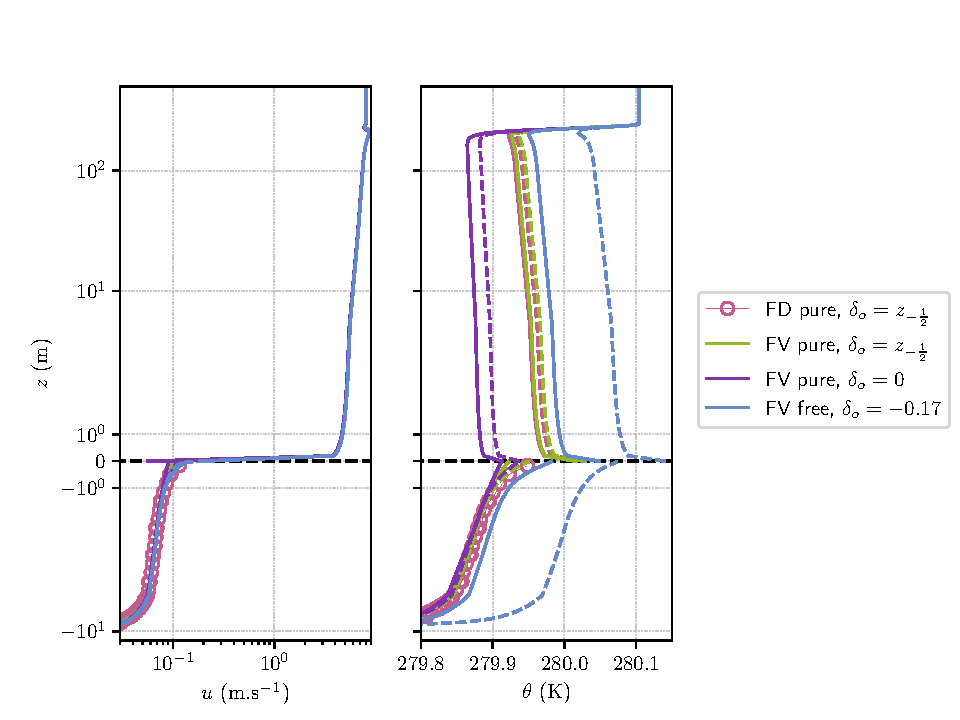
\includegraphics[scale=0.6]{images/oce_Coupled.pdf}
	\caption{Coupled case. The observed convergence factor
	of the Schwarz method was around $10^{-2}$.
	Dashed lines indicate
	a high resolution simulation and solid lines
	show the normal simulation.}
	\label{fig:OceanND_OSL_Coupled}
\end{figure}
\section{Partial conclusion}
No stability nor accuracy studies were conducted on these proposed
discretisations. Although they seem to behave correctly in the
experiments, further analyses of the "FV free" scheme are
necessary before they can be used. In particular,
the Finite Volume approximation between the first cell and the second
corresponds to the use of a strongly unstructured grid,
the second cell being typically twofold bigger than
the explicit part of the first cell.
% \subsubsection{Description of the two-sided bulk algorithm}
% \begin{equation}
% 	C_D^{a+o} = \left(\frac{\kappa} {
% 		\ln(1 + \frac{\delta_a}{z_{u}}) -
% 		\psi_m^a(\frac{\delta_a}{L_a})
% 		+ \lambda_u \left(
% 		\ln(1 - \frac{\delta_o}{z_{u}}) -
% 		\psi_m^o(-\frac{\delta_o}{L_o})
% 		\right)
% 	} \right)^2
% \end{equation}
% \begin{equation}
% 	C_H^{a+o} = \frac{\kappa \sqrt{C_D}} {
% 		\left(
% 			\ln(1 + \frac{\delta_a}{z_{\theta}}) -
% 			\psi_h^a(\frac{\delta_a}{L_a})
% 		\right)
% 		+
% 		(1 - \frac{Q_{lw}}
% 		{Q_H})
% 		\lambda_\theta \left(
% 			\ln(1 - \frac{\delta_o}{z_{\theta}}) -
% 			\psi_h^o(-\frac{\delta_o}{L_o})
% 		\right)
% 		- \frac{\lambda_\theta Q_{sw}(0)}
% 		{Q_H} E(\delta_o)
% 	}
% \end{equation}
% In the bulk algorithm, we use $u_a^\star = \sqrt{C_D} |u(\delta_a)-
% u(\delta_o)|$ and
% $\theta_a^\star = \frac{C_H}{\sqrt{C_D}}(\theta(\delta_a)-
% \theta(\delta_o))$ to get the friction scales.
% Multiplying those equations gives the boundary condition
% $K_\theta \partial_z \theta = \lambda_u \lambda_t u_a^\star \theta_a^\star$.
% \footnote{
% $u_a^\star$ is actually directly used because $\frac{C_H}{\sqrt{C_D}}$
% can be simplified.
% }
% We use the following notation for $C_D$ and $C_H$:
% \begin{equation}
% 	C_D^{a+o} = \frac{u_a^\star}{|u(\delta_a) - u(\delta_o)|},
% 	~~~
% 	C_D^{a} = \frac{u_a^\star}{|u(\delta_a) - u(0)|},
% 	~~~
% 	C_D^{o} = \frac{u_a^\star}{|u(0) - u(\delta_o)|},
% \end{equation}

